\newpage
\subsection{Cập nhật thông tin tài khoản}

\subsubsection*{Mục tiêu}
Chức năng cập nhật tài khoản cho phép người dùng chỉnh sửa thông tin cá nhân (họ tên, ngày sinh, địa chỉ, số điện thoại), cũng như thay đổi mật khẩu (passphrase). Việc này đảm bảo:
\begin{itemize}
    \item Người dùng có thể chủ động thay đổi thông tin cá nhân khi cần.
    \item Cho phép cập nhật passphrase và tự động mã hóa lại khóa RSA bằng passphrase mới.
    \item Đảm bảo tính bảo mật và tính nhất quán dữ liệu khóa trong hệ thống.
\end{itemize}

\subsubsection*{Giao diện}
Giao diện tại \texttt{/render\_update\_account} bao gồm:
\begin{itemize}
    \item Form nhập các trường: Họ tên, ngày sinh, địa chỉ, số điện thoại.
    \item Tùy chọn nhập mật khẩu hiện tại và mật khẩu mới nếu muốn đổi passphrase.
    \item Nút \texttt{Save changes} sẽ gửi POST đến API \texttt{/update\_account} và hiển thị thông báo kết quả.
\end{itemize}

\begin{figure}[H]
    \centering
    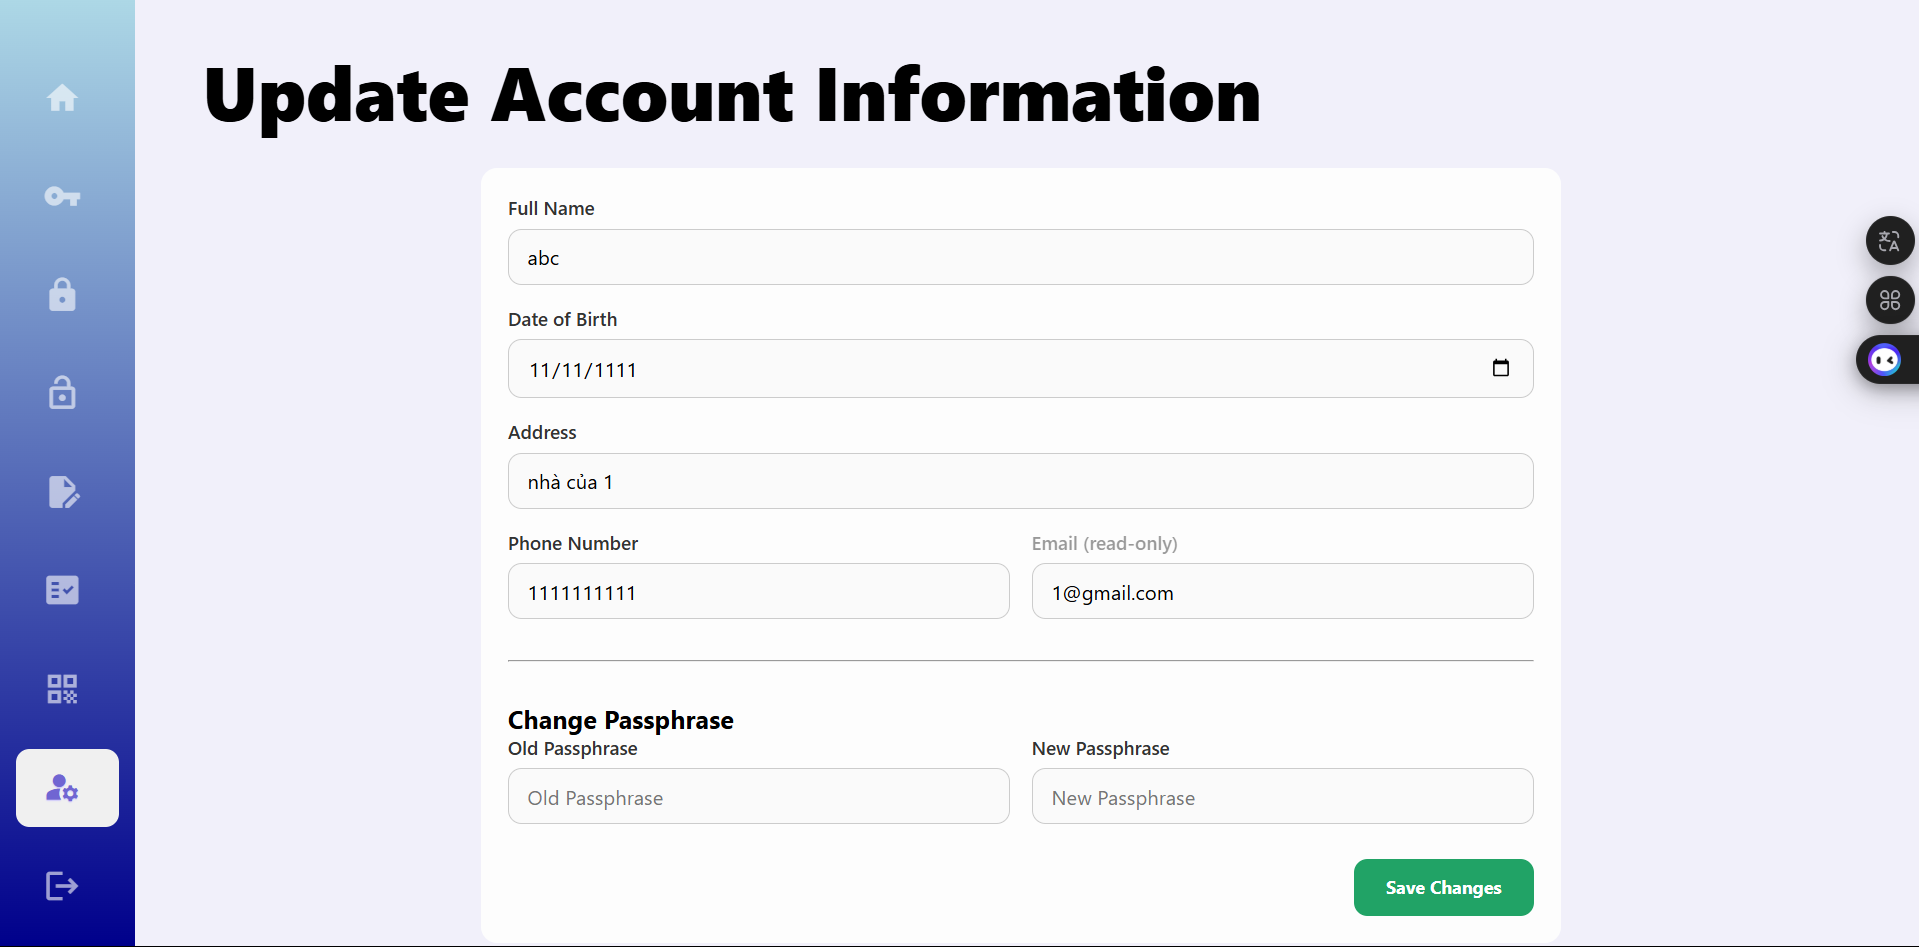
\includegraphics[width=0.85\textwidth]{img/5_update/5_update_form.png}
    \caption{Giao diện cập nhật thông tin}
\end{figure}

\subsubsection*{Quy trình thực hiện}
\begin{description}

    \item[\textbf{Bước 1 - Người dùng nhập thông tin}]
    Người dùng điền thông tin cần thay đổi, có thể chọn thay đổi passphrase hoặc không.

    \item[\textbf{Bước 2 - Gửi yêu cầu cập nhật}]
    Form gửi POST đến route \texttt{/update\_account}, kèm theo session để xác định người dùng.

    \item[\textbf{Bước 3 - Kiểm tra và xử lý}]
    Server thực hiện:
    \begin{itemize}
        \item Kiểm tra dữ liệu đầu vào và định dạng.
        \item Kiểm tra passphrase cũ nếu có yêu cầu đổi mật khẩu.
        \item Hash passphrase mới và cập nhật.
        \item Nếu đổi mật khẩu, khóa riêng RSA sẽ được giải mã bằng passphrase cũ và mã hóa lại bằng passphrase mới.
    \end{itemize}

    \item[\textbf{Bước 4 - Ghi log và phản hồi}]
    Ghi log cập nhật tài khoản và trả kết quả thành công hoặc thất bại cho giao diện frontend.

    \begin{figure}[H]
        \centering
        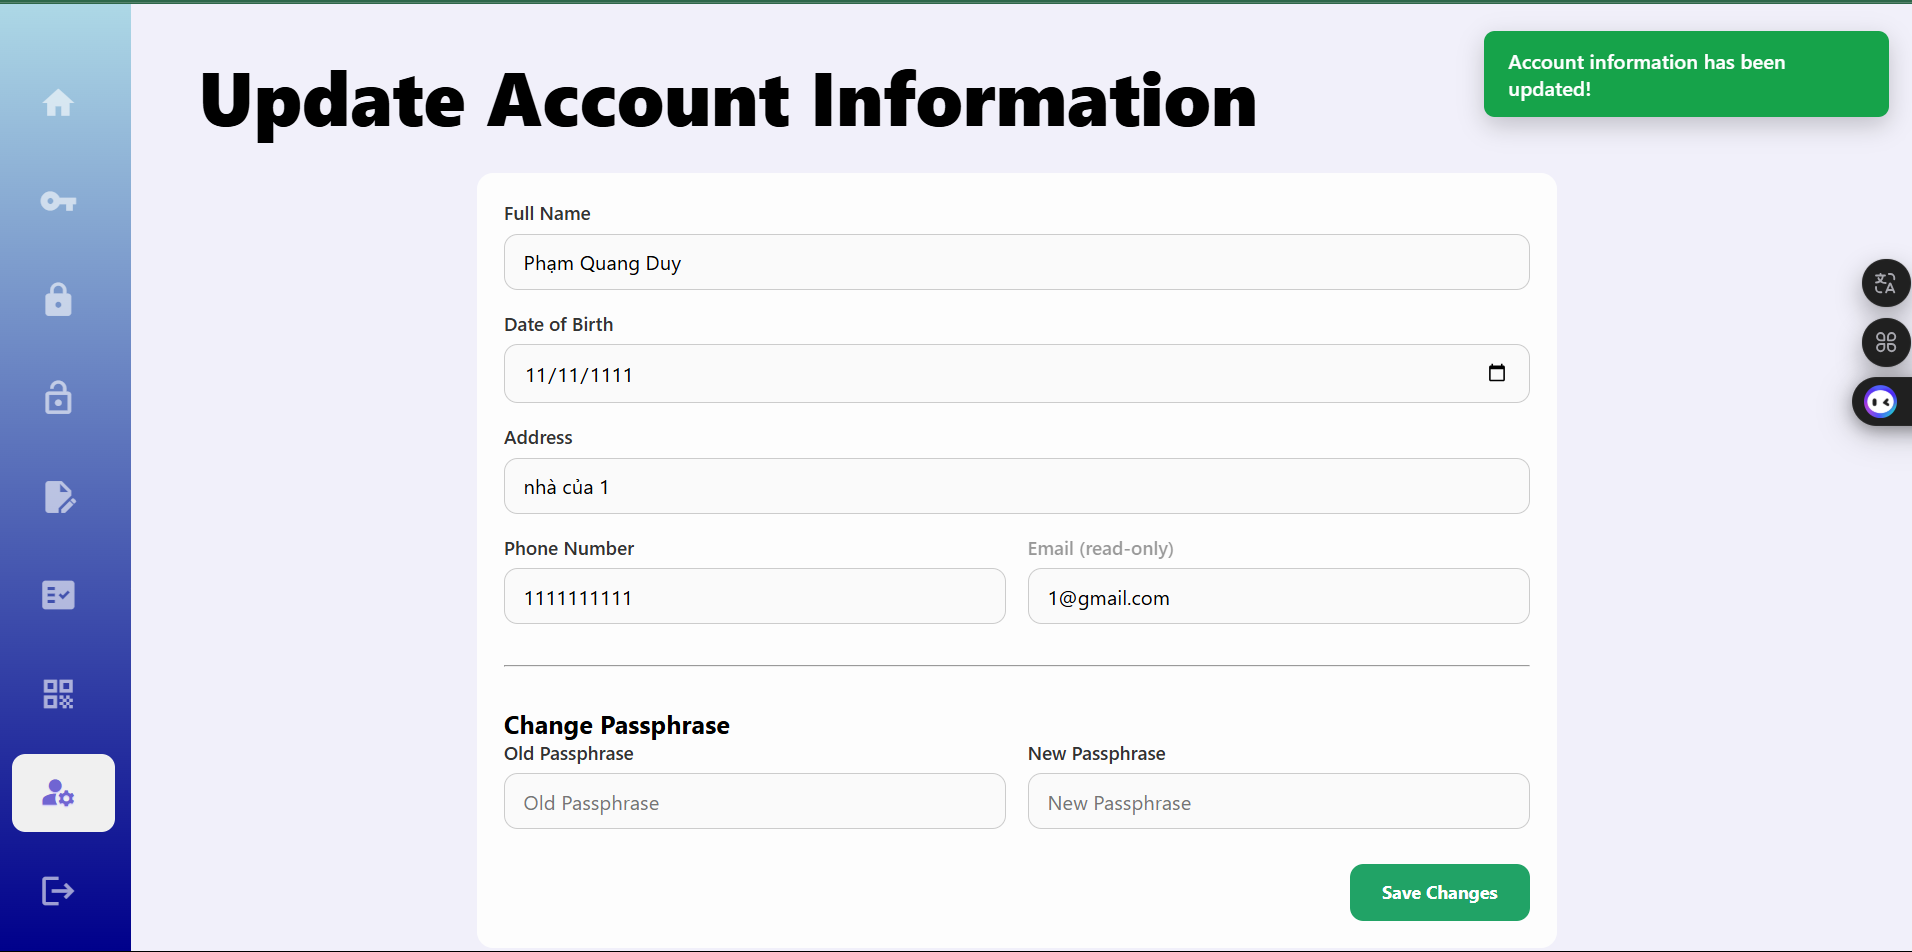
\includegraphics[width=0.85\textwidth]{img/5_update/5_update_success.png}
        \caption{Giao diện cập nhật thông tin thành công}
    \end{figure}
\end{description}

\subsubsection*{Chi tiết kỹ thuật và thư viện bảo mật}
\begin{description}

    \item[\textbf{1. Kiểm tra thông tin đầu vào}]
    \begin{itemize}
        \item Sử dụng các hàm xác thực định dạng: \texttt{is\_valid\_email()}, \texttt{is\_valid\_date()}, \texttt{is\_valid\_phone()}.
        \item Bắt buộc điền đầy đủ thông tin: email, họ tên, ngày sinh, địa chỉ, số điện thoại.
    \end{itemize}

    \item[\textbf{2. Kiểm tra và cập nhật passphrase}]
    \begin{itemize}
        \item Nếu có ý định đổi passphrase, yêu cầu nhập cả pass cũ và pass mới.
        \item Pass mới phải khác pass cũ và đạt yêu cầu bảo mật qua hàm \texttt{is\_strong\_passphrase()}.
        \item So sánh hash passphrase cũ với DB bằng \texttt{hash\_with\_salt()}.
        \item Nếu hợp lệ, hash passphrase mới và cập nhật vào DB.
    \end{itemize}

    \item[\textbf{3. Re-encrypt RSA key với passphrase mới}]
    \begin{itemize}
        \item Hàm \texttt{re\_encrypt\_private\_key\_with\_new\_passphrase()} dùng để giải mã khóa RSA bằng passphrase cũ và mã hóa lại bằng passphrase mới.
        \item Nếu lỗi trong quá trình này, cập nhật DB sẽ được rollback và trả lỗi.
        \item Passphrase mới được cập nhật vào session để sử dụng cho các thao tác sau.
    \end{itemize}
    \begin{figure}[H]
        \centering
        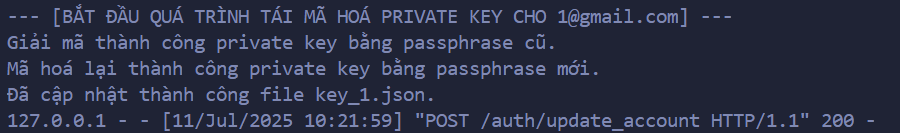
\includegraphics[width=0.85\textwidth]{img/5_update/5_update_re_enc.png}
        \caption{Mã hóa passphrase mới thành công}
    \end{figure}

    \item[\textbf{4. Cập nhật recovery key (khóa khôi phục)}]
    Để đảm bảo người dùng có thể khôi phục khóa riêng sau khi quên passphrase, hệ thống sử dụng một \textbf{recovery key} (AES key phụ) được mã hóa bằng passphrase hiện tại. Khi người dùng thay đổi passphrase, recovery key cần được giải mã và mã hóa lại như sau:

    \begin{itemize}
        \item \textbf{Bước 1: Giải mã recovery key bằng passphrase cũ}
        \begin{itemize}
            \item Truy vấn trường \texttt{encrypted\_recovery\_key} từ bảng \texttt{users}.
            \item Derive khóa AES từ passphrase cũ bằng hàm \texttt{derive\_aes\_key(pass1, salt)}.
            \item Giải mã recovery key hiện tại bằng AES.
        \end{itemize}

        \item \textbf{Bước 2: Mã hóa lại recovery key bằng passphrase mới}
        \begin{itemize}
            \item Derive AES key mới từ passphrase mới: \texttt{derive\_aes\_key(pass2, salt)}.
            \item Mã hóa recovery key vừa giải mã bằng AES key mới.
            \item Lưu bản mã hóa mới vào trường \texttt{encrypted\_recovery\_key}.
        \end{itemize}

        \item \textbf{Lưu ý bảo mật:}
        \begin{itemize}
            \item Nếu giải mã hoặc mã hóa recovery key thất bại, toàn bộ quá trình cập nhật sẽ bị rollback và trả lỗi.
            \item Mọi thao tác đều được log bằng \texttt{log\_user\_action(..., "Fail", ...)} hoặc \texttt{log\_internal\_event()} với mức \texttt{error}.
        \end{itemize}
    \end{itemize}

    \item[\textbf{5. Ghi log và bảo mật}]
    \begin{itemize}
        \item Mọi thao tác đều được ghi bằng \texttt{log\_user\_action()} với trạng thái và chi tiết lỗi.
        \item Lỗi truy cập không có session sẽ chuyển hướng về trang đăng nhập.
        \item Dữ liệu passphrase luôn được hash bằng salt, không lưu dưới dạng thô.
    \end{itemize}

    \item[\textbf{6. Xử lý lỗi}]
    \begin{itemize}
        \item Nếu thiếu session → lỗi 401 hoặc redirect về trang đăng nhập.
        \item Nếu định dạng sai hoặc passphrase cũ không đúng → trả lỗi rõ ràng.
        \item Nếu không có thay đổi gì → trả thông báo: \texttt{"No changes were made."}
        \item Nếu cập nhật thành công nhưng RSA re-encryption thất bại → rollback và log lỗi mức độ \texttt{error}.
    \end{itemize}

    
    \begin{figure}[H]
        \centering
        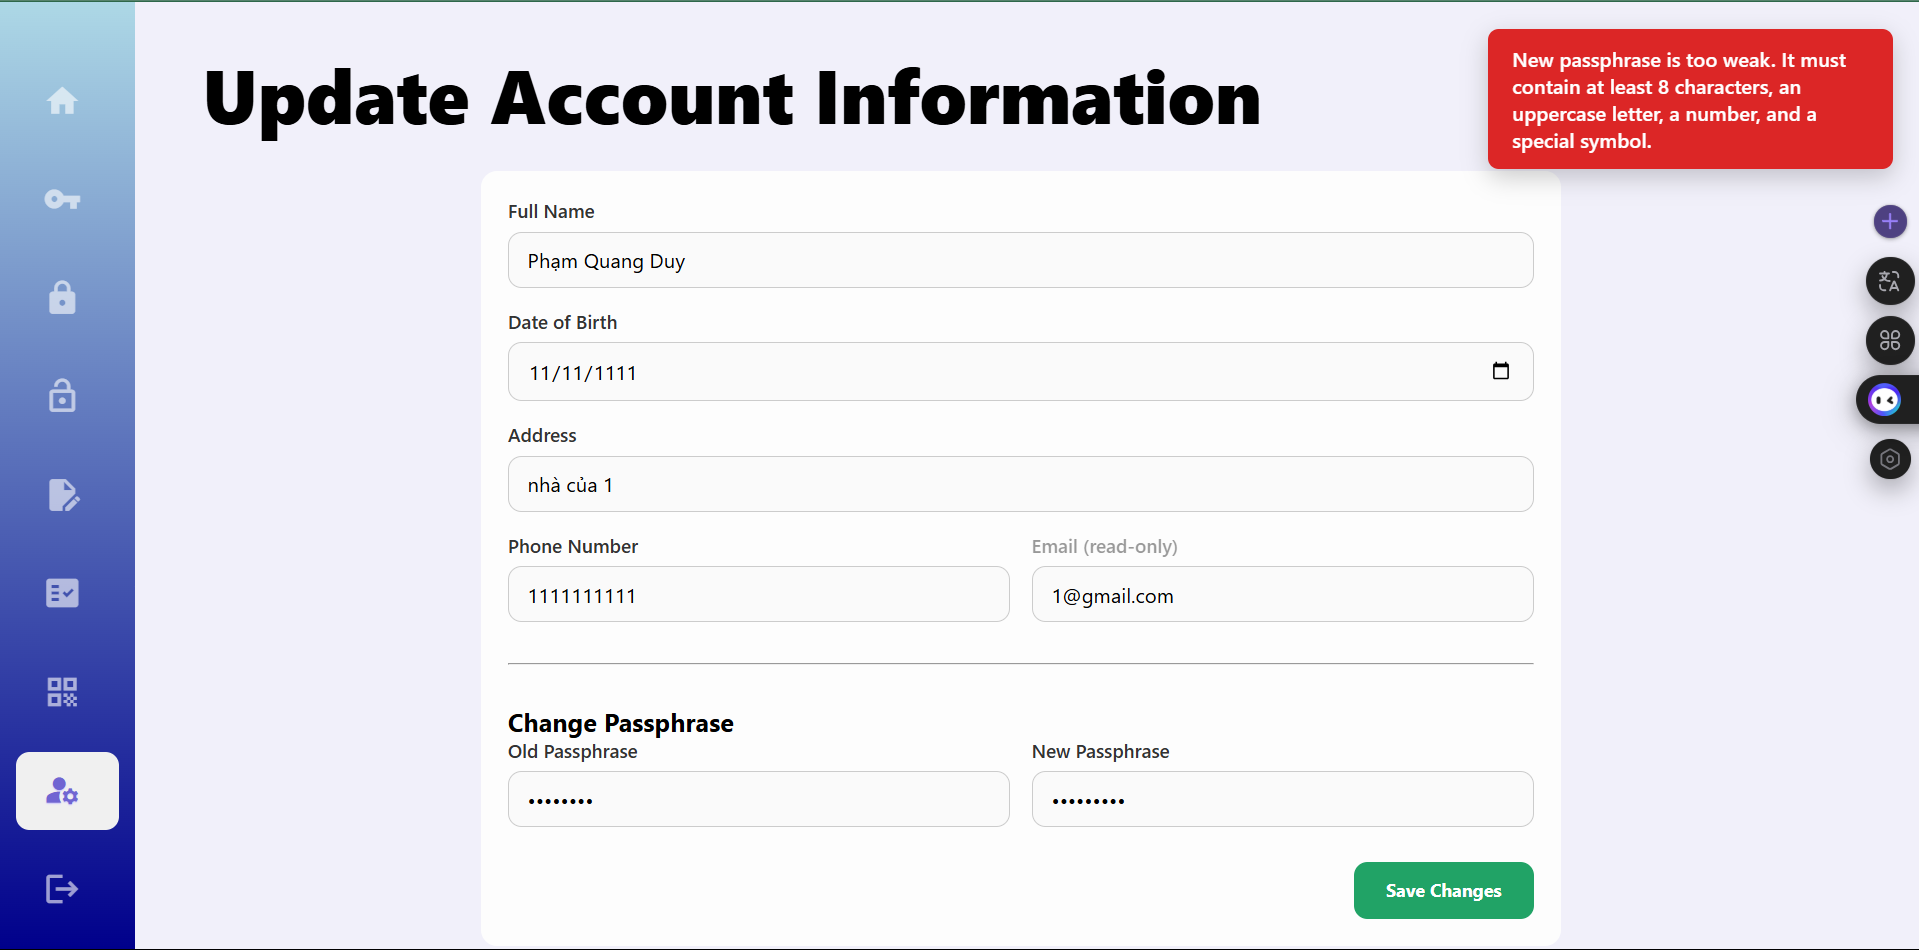
\includegraphics[width=0.85\textwidth]{img/5_update/5_update_fail_1.png}
        \caption{Thông báo lỗi khi kiểm tra đầu vào}
    \end{figure}

    \begin{figure}[H]
        \centering
        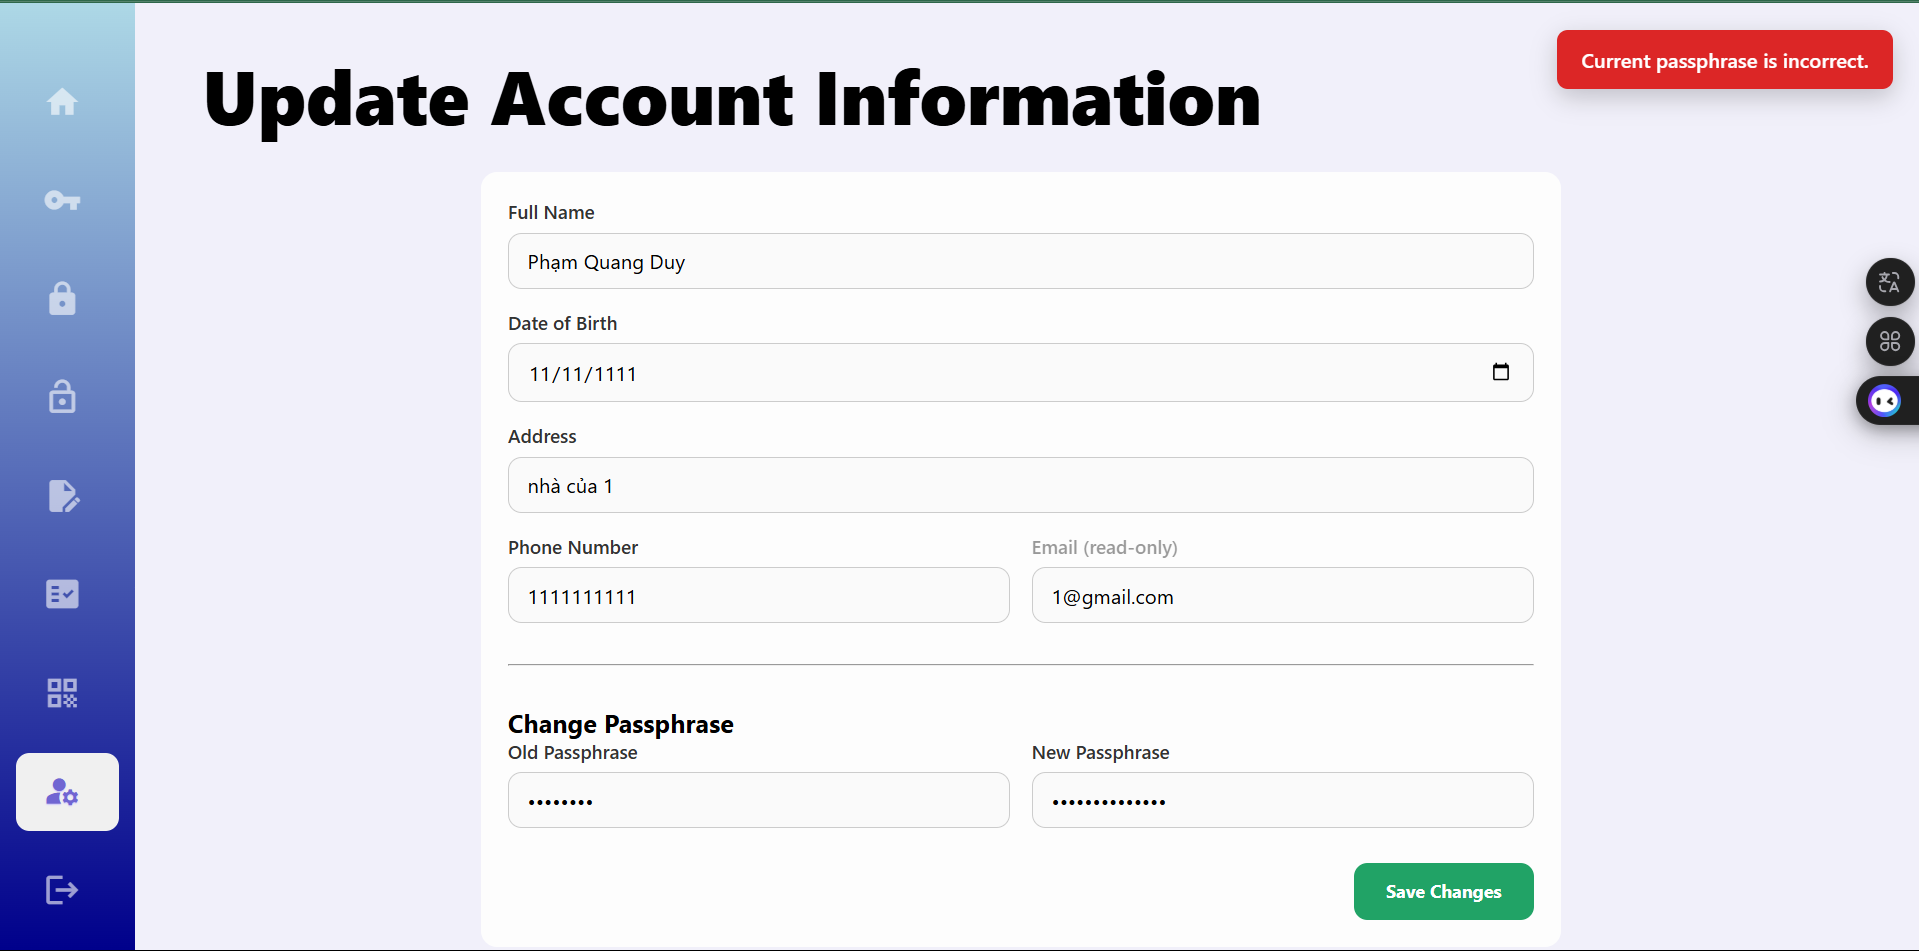
\includegraphics[width=0.85\textwidth]{img/5_update/5_update_fail_2.png}
        \caption{Thông báo lỗi khi kiểm tra đầu vào}
    \end{figure}

    \begin{figure}[H]
        \centering
        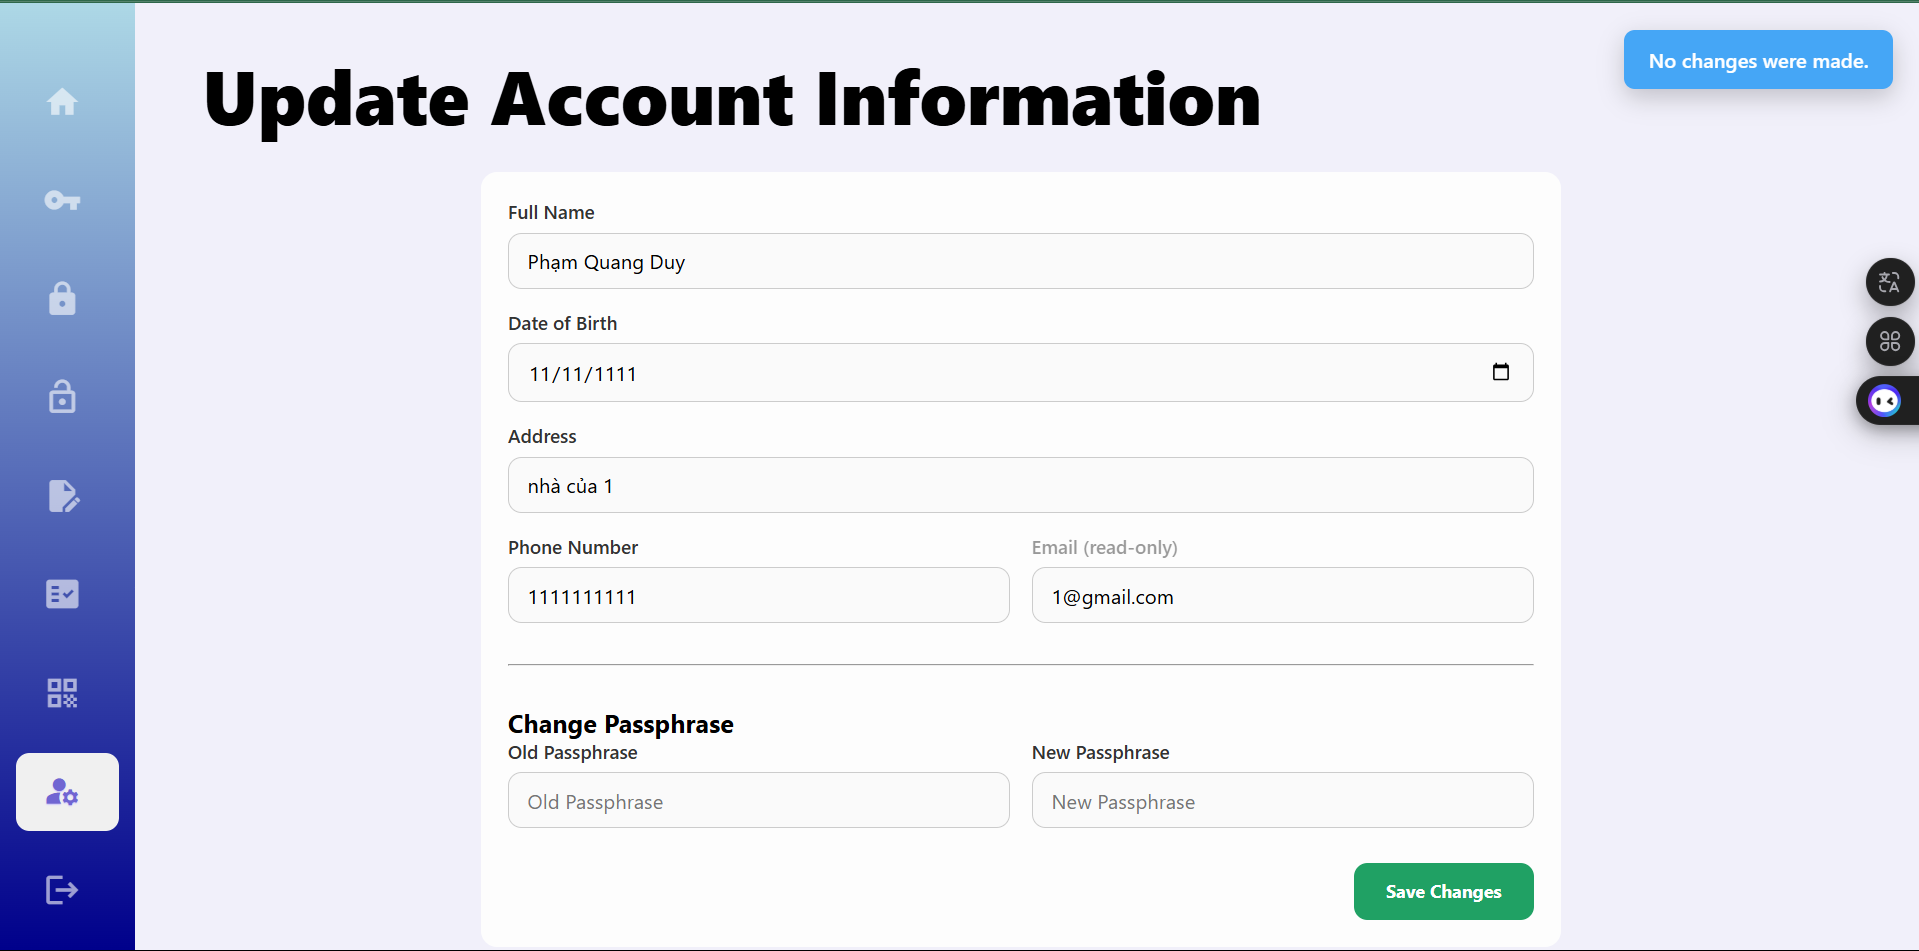
\includegraphics[width=0.85\textwidth]{img/5_update/5_update_no_changes.png}
        \caption{Thông báo khi không có thay đổi}
    \end{figure}
\end{description}
